\begin{figure}[H]
\centering
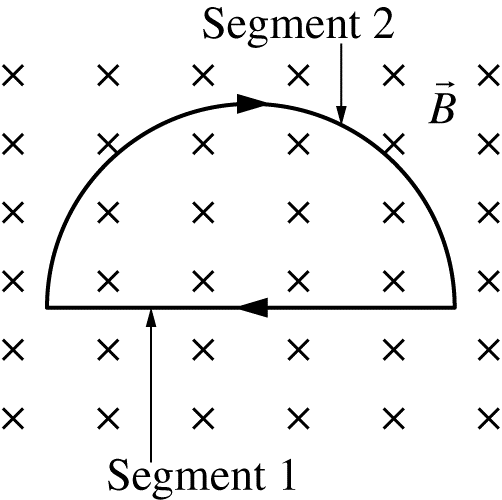
\includegraphics[scale=0.3]{images/img-016-024.png}
\end{figure}

% Multiple Choice Question 35
\begin{questions}\setcounter{question}{34}\question
A semicircular loop with a clockwise current is placed in a uniform magnetic field that is directed into the page, as shown in the figure above. $\vec{F}_{1}$ is the net force on segment 1 , the straight portion of the loop. $\vec{F}_{2}$ is the net force on segment 2 , the curved portion of the loop. Which of the following correctly indicates the directions and relative magnitudes of the forces $\vec{F}_{1}$ and $\vec{F}_{2}$ ?

\tabto{ 0.75cm} \underline{Direction of $\vec{F}_{1}$}
\tabto{ 7.00cm} \underline{Direction of $\vec{F}_{2}$}
\tabto{13.25cm} \underline{Magnitudes}

\begin{choices}
\choice
    Toward the bottom of the page
    \tabto{6.25cm} Toward the top of the page
    \tabto{12.50cm} $\abs{\vec{F}_{1}} = \abs{\vec{F}_{2}}$
\choice
    Toward the bottom of the page
    \tabto{6.25cm} Toward the top of the page
    \tabto{12.50cm} $\abs{\vec{F}_{1}} < \abs{\vec{F}_{2}}$
\choice
    Toward the bottom of the page
    \tabto{6.25cm} Toward the top of the page
    \tabto{12.50cm} $\abs{\vec{F}_{1}} > \abs{\vec{F}_{2}}$
\choice
    Toward the top of the pag
    \tabto{6.25cm} Toward the bottom of the page
    \tabto{12.50cm} $\abs{\vec{F}_{1}} = \abs{\vec{F}_{2}}$
\choice
    Toward the top of the pag
    \tabto{6.25cm} Toward the bottom of the page
    \tabto{12.50cm} $\abs{\vec{F}_{1}} < \abs{\vec{F}_{2}}$
\end{choices}\end{questions}
